\documentclass[a4paper]{article}

\usepackage{inputenc}
\usepackage[british,UKenglish]{babel}
\usepackage{amsmath}
%\usepackage{titlesec}
\usepackage{color}
\usepackage{graphicx}
\usepackage{fancyref}
\usepackage{hyperref}
\usepackage{float}
\usepackage{scrextend}
\usepackage{setspace}
\usepackage{xargs}
\usepackage{multicol}
\usepackage{nameref}

\usepackage{sectsty}
\usepackage{multicol}
\usepackage{multirow}
\usepackage[procnames]{listings}
\usepackage{appendix}

\newcommand\tab[1][1cm]{\hspace*{#1}}
\hypersetup{colorlinks=true, linkcolor=black}
\interfootnotelinepenalty=10000

\newcommand{\cleancode}[1]{\begin{addmargin}[3em]{3em}\texttt{\textcolor{cleanOrange}{#1}}\end{addmargin}}
\newcommand{\cleanstyle}[1]{\text{\textcolor{cleanOrange}{\texttt{#1}}}}


\usepackage[colorinlistoftodos,prependcaption,textsize=footnotesize]{todonotes}
\newcommandx{\commred}[2][1=]{\textcolor{Red}
{\todo[linecolor=red,backgroundcolor=red!25,bordercolor=red,#1]{#2}}}
\newcommandx{\commblue}[2][1=]{\textcolor{Blue}
{\todo[linecolor=blue,backgroundcolor=blue!25,bordercolor=blue,#1]{#2}}}
\newcommandx{\commgreen}[2][1=]{\textcolor{OliveGreen}{\todo[linecolor=OliveGreen,backgroundcolor=OliveGreen!25,bordercolor=OliveGreen,#1]{#2}}}
\newcommandx{\commpurp}[2][1=]{\textcolor{Plum}{\todo[linecolor=Plum,backgroundcolor=Plum!25,bordercolor=Plum,#1]{#2}}}

\def\code#1{{\tt #1}}

\def\note#1{\noindent{\bf [Note: #1]}}

\makeatletter
%% The "\@seccntformat" command is an auxiliary command
%% (see pp. 26f. of 'The LaTeX Companion,' 2nd. ed.)
\def\@seccntformat#1{\@ifundefined{#1@cntformat}%
   {\csname the#1\endcsname\quad}  % default
   {\csname #1@cntformat\endcsname}% enable individual control
}
\let\oldappendix\appendix %% save current definition of \appendix
\renewcommand\appendix{%
    \oldappendix
    \newcommand{\section@cntformat}{\appendixname~\thesection\quad}
}
\makeatother


% "define" Scala
\usepackage[T1]{fontenc}  
\usepackage[scaled=0.82]{beramono}  
\usepackage{microtype} 

\sbox0{\small\ttfamily A}
\edef\mybasewidth{\the\wd0 }

\lstdefinelanguage{scala}{
  morekeywords={abstract,case,catch,class,def,%
    do,else,extends,false,final,finally,%
    for,if,implicit,import,match,mixin,%
    new,null,object,override,package,%
    private,protected,requires,return,sealed,%
    super,this,throw,trait,true,try,%
    type,val,var,while,with,yield},
  sensitive=true,
  morecomment=[l]{//},
  morecomment=[n]{/*}{*/},
  morestring=[b]",
  morestring=[b]',
  morestring=[b]"""
}

\usepackage{color}
\definecolor{dkgreen}{rgb}{0,0.6,0}
\definecolor{gray}{rgb}{0.5,0.5,0.5}
\definecolor{mauve}{rgb}{0.58,0,0.82}

% Default settings for code listings
\lstset{frame=tb,
  language=scala,
  aboveskip=3mm,
  belowskip=3mm,
  showstringspaces=false,
  columns=fixed, % basewidth=\mybasewidth,
  basicstyle={\small\ttfamily},
  numbers=none,
  numberstyle=\footnotesize\color{gray},
  % identifierstyle=\color{red},
  keywordstyle=\color{blue},
  commentstyle=\color{dkgreen},
  stringstyle=\color{mauve},
  frame=single,
  breaklines=true,
  breakatwhitespace=true,
  procnamekeys={def, val, var, class, trait, object, extends},
  procnamestyle=\ttfamily\color{red},
  tabsize=2
}

\lstnewenvironment{scala}[1][]
{\lstset{language=scala,#1}}
{}
\lstnewenvironment{cpp}[1][]
{\lstset{language=C++,#1}}
{}
\lstnewenvironment{bash}[1][]
{\lstset{language=bash,#1}}
{}
\lstnewenvironment{verilog}[1][]
{\lstset{language=verilog,#1}}
{}



%代码段设置
\lstset{numbers=left,
basicstyle=\tiny,
numberstyle=\tiny,
keywordstyle=\color{blue!70},
commentstyle=\color{red!50!green!50!blue!50},
frame=single, rulesepcolor=\color{red!20!green!20!blue!20},
escapeinside=``
}

\graphicspath{ {figures/} }
\usepackage{ctex}
\setCJKmainfont[ItalicFont=Noto Sans CJK SC Bold, BoldFont=Noto Serif CJK SC Black]{Noto Serif CJK SC}
\usepackage{graphicx}
\usepackage{color,framed}%文本框
\usepackage{listings}
\usepackage{caption}
\usepackage{amssymb}
\usepackage{enumerate}
\usepackage{xcolor}
\usepackage{bm} 
\usepackage{lastpage}%获得总页数
\usepackage{fancyhdr}
\usepackage{tabularx}  
\usepackage{geometry}
\usepackage{minted}
\usepackage{graphics}
\usepackage{subfigure}
\usepackage{float}
\usepackage{pdfpages}
\usepackage{pgfplots}
\pgfplotsset{width=10cm,compat=1.9}
\usepackage{multirow}
\usepackage{footnote}
\usepackage{booktabs}

%-----------------------伪代码------------------
\usepackage{algorithm}  
\usepackage{algorithmicx}  
\usepackage{algpseudocode}  
\floatname{algorithm}{Algorithm}  
\renewcommand{\algorithmicrequire}{\textbf{Input:}}  
\renewcommand{\algorithmicensure}{\textbf{Output:}} 
\usepackage{lipsum}  
\makeatletter
\newenvironment{breakablealgorithm}
  {% \begin{breakablealgorithm}
  \begin{center}
     \refstepcounter{algorithm}% New algorithm
     \hrule height.8pt depth0pt \kern2pt% \@fs@pre for \@fs@ruled
     \renewcommand{\caption}[2][\relax]{% Make a new \caption
      {\raggedright\textbf{\ALG@name~\thealgorithm} ##2\par}%
      \ifx\relax##1\relax % #1 is \relax
         \addcontentsline{loa}{algorithm}{\protect\numberline{\thealgorithm}##2}%
      \else % #1 is not \relax
         \addcontentsline{loa}{algorithm}{\protect\numberline{\thealgorithm}##1}%
      \fi
      \kern2pt\hrule\kern2pt
     }
  }{% \end{breakablealgorithm}
     \kern2pt\hrule\relax% \@fs@post for \@fs@ruled
  \end{center}
  }
\makeatother
%------------------------代码-------------------
\usepackage{xcolor} 
\usepackage{listings} 
\lstset{ 
breaklines,%自动换行
basicstyle=\small,
escapeinside=``,
keywordstyle=\color{ blue!70} \bfseries,
commentstyle=\color{red!50!green!50!blue!50},% 
stringstyle=\ttfamily,% 
extendedchars=false,% 
linewidth=\textwidth,% 
numbers=left,% 
numberstyle=\tiny \color{blue!50},% 
frame=trbl% 
rulesepcolor= \color{ red!20!green!20!blue!20} 
}

%-------------------------页面边距--------------
\geometry{a4paper,left=2.3cm,right=2.3cm,top=2.7cm,bottom=2.7cm}
%-------------------------页眉页脚--------------
\usepackage{fancyhdr}
\pagestyle{fancy}
\lhead{\kaishu \leftmark}
% \chead{}
\rhead{\kaishu 并行程序设计期末研究报告}%加粗\bfseries 
\lfoot{}
\cfoot{\thepage}
\rfoot{}
\renewcommand{\headrulewidth}{0.1pt}  
\renewcommand{\footrulewidth}{0pt}%去掉横线
\newcommand{\HRule}{\rule{\linewidth}{0.5mm}}%标题横线
\newcommand{\HRulegrossa}{\rule{\linewidth}{1.2mm}}
\setlength{\textfloatsep}{10mm}%设置图片的前后间距
%--------------------文档内容--------------------

\begin{document}
\renewcommand{\contentsname}{目\ 录}
\renewcommand{\appendixname}{附录}
\renewcommand{\appendixpagename}{附录}
\renewcommand{\refname}{参考文献}
\renewcommand{\figurename}{图}
\renewcommand{\tablename}{表}
\renewcommand{\today}{\number\year 年 \number\month 月 \number\day 日}

%-------------------------封面----------------
\begin{titlepage}
  \begin{center}
    
\includegraphics[width=0.8\textwidth]{NKU.png}\\[1cm]
    \vspace{20mm}
    \textbf{\huge\textbf{\kaishu{计算机学院}}}\\[0.5cm]
    \textbf{\huge{\kaishu{并行程序设计}}}\\[2.3cm]
    \textbf{\Huge\textbf{\kaishu{特殊高斯消去法的并行优化}}}

    \vspace{\fill}

    \textbf{\Large \textbf{并行程序设计期末研究报告}}\\[0.8cm]
    \HRule \\[0.9cm]
    \HRule \\[2.0cm]
    \centering
    \textsc{\LARGE \kaishu{姓名\ :\ 丁屹、卢麒萱}}\\[0.5cm]
    \textsc{\LARGE \kaishu{学号\ :\ 2013280、2010519}}\\[0.5cm]
    \textsc{\LARGE \kaishu{专业\ :\ 计算机科学与技术}}\\[0.5cm]

    \vfill
    {\Large \today}
  \end{center}
\end{titlepage}

\renewcommand {\thefigure}{\thesection{}.\arabic{figure}}%图片按章标号
\renewcommand{\figurename}{图}
\renewcommand{\contentsname}{目录}
\cfoot{\thepage\ of \pageref{LastPage}}%当前页 of 总页数


% 生成目录
\clearpage
\tableofcontents
\newpage

\section{问题描述}
\subsection{普通高斯消去法}
普通高斯消去的计算模式如图 \ref{gauss} 所示,在第$k$步时,对第$k$行从$(k, k)$开始进行除法操作,并且将后续的$k + 1$至$N$行进行减去第$k$行的操作,串行算法如下面伪代码所示。
\begin{figure}
  \centering
  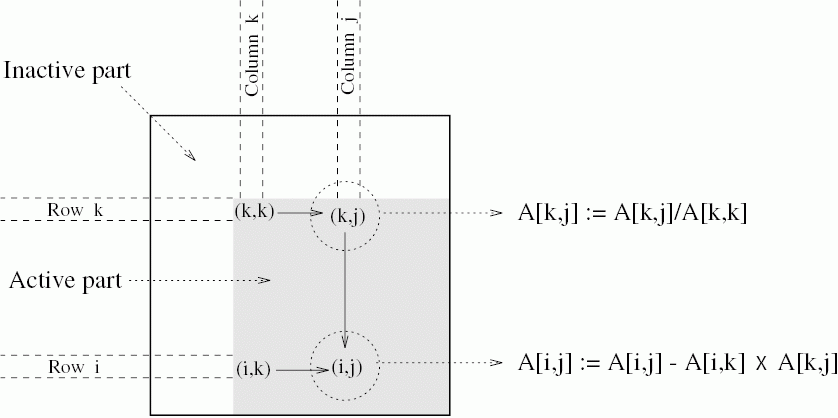
\includegraphics[width=1\textwidth]{gauss.png}
  \caption{高斯消去法示意图}
  \label{gauss}
\end{figure}
\begin{breakablealgorithm}
  \caption{普通高斯消元算法伪代码}
  \begin{algorithmic}[1] %每行显示行号  
    \Function {LU}{}
    \For {$k:=0$\ \textbf{to}\ $n$}
    \For {$j:=k+1$\ \textbf{to}\ $n$}
    \State {$A[k,j]:=A[k,j]/A[k,k]$}
    \EndFor
    \State{$A[k,k]:=1.0$}
    \For {$i:=k+1$\ \textbf{to}\ $n$}
    \For {$j:=k+1$\ \textbf{to}\ $n$}
    \State {$A[i,j]:=A[i,j]-A[i,k]*A[k,j]$}
    \EndFor
    \State{$A[i,k]:=0$}
    \EndFor
    \EndFor
    \EndFunction
  \end{algorithmic}
\end{breakablealgorithm}

\subsection{特殊高斯消去法}
本算法源自布尔 Gröbner 基计算。
Gröbner基是一种广泛应用于复杂高次方程体系的计算方法,它是 Buchberger首先提出的。它的实质是从多项式环的任何一个理想的生成元上,对一组“好的”生成元进行描述和计算,从而对理想的构造进行分析,并对其进行一些理想的运算。由于数学、科学和工程学中的许多问题都可以用多元多项式方程组表示(例如,理想,模块和矩阵),Gröbner基的代数算法在理论物理学、应用科学和工程学中具有广泛的应用。
在 HFE80 的 Gröbner 基计算过程中,高斯消元时间占比可以达到90\% 以上。考虑到此算法中高斯消元的特殊性,为加快高斯消元速度,设计此算法。
\subsubsection{符号说明}
$R$:所有消元子构成的集合

$R[i]$:首项为 $i$ 的消元子

$E$:所有被消元行构成的数组

$E[i]$:第 $i$ 个被消元行

$lp(E[i])$:被消元行第 $i$ 行的首项

这里首项的含义:首项是指某行下标最大的非零项的下标,如某行为 011000,从左到右下标分别为 5,4,3,2,1,0,那么首项为 4,因为该行非零项下标为 3,4,其中最大值为 4。

\subsubsection{算法伪代码}
\begin{breakablealgorithm}
  \caption{串行算法伪代码}
  \begin{algorithmic}[1] %每行显示行号  
    \Function {Gauss}{}
    \For {$i:=0$\ \textbf{to}\ $m-1$}
    \While {$E[i]!=0$}
    \If{$R[lp(E[i])]!=NULL$}
    \State $E[i]:=E[i]−R[lp(E[i])]$
    \Else\State{$R[lp(E[i])]:=E[i]$}
    \State\textbf{break}
    \EndIf
    \EndWhile
    \EndFor
    \State \Return{$E$}
    \EndFunction
  \end{algorithmic}
\end{breakablealgorithm}

在这里,最外层循环代表了对每一个被消元的行的遍历。内层循环代表每一条被消元行,若行没有被消为0,则按照其第一项选择消元;如果有适当的消元符,则用该消元子消元,或者将该被消元行作为消元子,参加下一步的高斯消元。

\subsubsection{数据结构}
可采用位向量方式存储每个消元子和被消元行,优点是消元操作变为位向量异或操作,算法实现简单,且适合并行化,易达到更高的并行效率,缺点是 Gröbner 基计算中产生的消元子和被消元行非常稀疏,非零元素( 1 元素)在 5 \% 以下,位向量存储和计算可能并非最优。
也可采用类似倒排链表的存储及方式——可认为是稀疏 0 / 1 矩阵的紧凑存储方式,每个消元子和被消元行只保存1元素的位置,且按升序排列,从而类似倒排链表数据结构。优点是存储空间占用更少,缺点是算法设计更复杂,并行化难度高。


\section{研究设计}
项目链接:
\url{https://github.com/NeoWans/Parallel-Programming-Final}

\subsection{测试用例}
测试用例由老师提供的Groebner.7z压缩包解压后获得,总共11组数据,软链接至res/目录下,命名规则为\%组号\%.0 (非零消元子)、\%组号\%.1 (被消元行)、\%组号\%.2 (消元结果)

\subsection{实验环境和相关配置}
实验在本地 x86 Arch Linux 环境下完成,使用 Makefile 构建项目,开启 Ofast 加速;
使用的 CPU 为 AMD Ryzen 4800HS (8C16T),系统 RAM 大小为 38.6G,显卡为 nVIDIA RTX 2060 6G。

\subsection{串行倒排链表算法}
使用STL list存储矩阵中每行的非零位置,逐行放入嵌套的外层STL list;
使用STL map存储消元行首项与消元行的映射。

\begin{lstlisting}[frame=trbl, language={C++}, caption={串行倒排链表消元部分}]
void gauss(list_matrix_t& m) {
  for (auto& eliminatee : m.op) {
    while (!eliminatee.empty()) {
      auto  key        = *(eliminatee.cbegin());
      auto& eliminater = m.pool[key];
      if (eliminater.empty()) {
        eliminater = eliminatee;
        break;
      } else {
        auto jt = eliminatee.begin();
        auto it = eliminater.cbegin();
        while (it != eliminater.cend() && jt != eliminatee.end())
          if (*it > *jt) eliminatee.insert(jt, *it++);
          else if (*it == *jt) jt = eliminatee.erase(jt), ++it;
          else ++jt;
        for (; it != eliminater.cend(); ++it) eliminatee.push_back(*it);
      }
    }
  }
}
\end{lstlisting}

\subsection{串行位元矩阵算法}
使用STL bitset倒序存储矩阵每行,逐行放入外层STL list;
使用STL map存储消元行首项与消元行的映射。

其中值得注意的是,STL bitset提供了快速查询最低真值位索引的内建成员函数\_Find\_first(),与之对应的是算法需要$lp(E[i])$操作,即获得被消元行第i行的首项,然而正序存储时\_Find\_first函数得到的是被消元行第i行的末项,因此需要倒序存储。具体实现使用了"bsmap"宏 \ref{code:bsmap} 处理映射关系。由于STL bitset需要使用常量模板参数声明,因此使用了 "matrix\_max\_sz" 常量,大小为 85401,即测试样例中的最大矩阵大小。bsmap可以保证定义域和陪域在 $[0, matrix\_max\_sz)$ 内且为双射,同时满足 $\forall{x \in [0, matrix\_max\_sz)}\ bsmap(bsmap(x)) = x$。
\begin{lstlisting}[frame=trbl, language={C++}, caption={bsmap 宏}, label = {code:bsmap}]
#define bsmap(i) (matrix_max_sz - 1 - (i))
\end{lstlisting}

\begin{lstlisting}[frame=trbl, language={C++}, caption={串行位元矩阵消元部分}]
void gauss(bitset_matrix_t& m) {
  for (auto& eliminatee : m.op) {
    while (eliminatee.any()) {
      auto  key        = bsmap(eliminatee._Find_first());
      auto& eliminater = m.pool[key];
      if (eliminater.none()) {
        eliminater = eliminatee;
        break;
      } else eliminatee ^= eliminater;
    }
  }
}
\end{lstlisting}

\subsection{并行倒排链表算法}
由于分析测试数据发现使用链表存储矩阵运行时间远大于bitset存储,常数过大,即使在稀疏矩阵下也仅有内存占用低的优势。然而并行位元矩阵算法在稀疏矩阵下的内存占用也是完全可以接受的,没有研究的必要。

\subsection{并行位元矩阵算法}
使用STL bitset倒序存储矩阵每行,逐行放入外层数组;
由于矩阵的秩比较小,而且测试样例存在稠密矩阵,所以决定改用数组存储消元行首项与消元行的映射。

并行化库选择了C++11的标准库thread,可以最大程度保证可移植性。并发线程数量读取thread::hardware\_concurrency()的提示,在本地机器上为16。

经过观察可以发现,外层循环就是并行化改造的入手点。这里采取了按照循环划分的方法,将线程id与行对线程总数的模数对应。由于存在被消元子成为非零消元子的可能,非零消元子不是只读访问。因此使用可升级的读写锁最符合直觉。即访问非零消元子前需要获取读锁,如果需要对消元子复制,则将读锁升级为写锁。这样借助boost::upgrade\_lock就有了一种使用读写锁实现 \ref{code:upgrade-lock},具体来说,其中:boost::upgrade\_lock<boost::shared\_mutex>实现加读锁,boost::upgrade\_to\_unique\_lock<boost::shared\_mutex>实现将读锁升级为写锁。

\begin{lstlisting}[frame=trbl, language={C++}, caption={upgrade\_lock 位元矩阵消元部分}, label={code:upgrade-lock}]
  const auto num_thread = thread::hardware_concurrency();
  boost::shared_mutex mutex_main;
  void thread_callback(size_t index, bitset_matrix_t& m) {
    for (size_t local_index = index; local_index < m.op.size();
         local_index += num_thread) {
      auto& eliminatee = m.op.at(local_index);
      while (eliminatee.any()) {
        auto key = bsmap(eliminatee._Find_first());
        boost::upgrade_lock<boost::shared_mutex> read_lock(mutex_main);
        auto&                                    eliminater = m.pool[key];
        if (eliminater.none()) {
          boost::upgrade_to_unique_lock<boost::shared_mutex> write_lock(
            read_lock);
          eliminater = eliminatee;
          break;
        } else eliminatee ^= eliminater;
      }
    }
  }
  void gauss(bitset_matrix_t& m) {
    list<thread> thread_pool;
    for (unsigned i = 0; i < num_thread; ++i)
      thread_pool.push_back(thread(thread_callback, i, ref(m)));
    for (auto& t : thread_pool) t.join();
  }
\end{lstlisting}

然而经过测试,这种实现的计算效率甚至不如串行算法(表\ref{tab:thread}),因此有了下面的 call\_once 实现。

再次观察可以注意到,实际上映射数组里的每一种消元子只会被初始化一次,能够对应保证线程安全的前提下初始化单例类型的模型,即双重检查锁定模型。换言之存在减少加锁次数提高性能的优化空间。对于支持 C++11 以上的编译器,存在 call\_once 和 once\_flag 原语。对call\_once传入once\_flag标志和回调函数func即可实现线程安全的前提下仅第一次成功调用回调函数func。称为"积极调用",并对once\_flag翻转;此后再次向call\_once传入once\_flag就直接返回,称为"消极调用"。避免了双重检查锁定模型的繁琐和危险。因此我们有了另一种不使用boost的更快的实现 \ref{code:call-once}。

\begin{lstlisting}[frame=trbl, language={C++}, caption={call\_once 位元矩阵消元部分}, label={code:call-once}]
const auto num_thread = thread::hardware_concurrency();

void thread_callback(size_t index, bitset_matrix_t& m) {
  for (size_t local_index = index; local_index < m.op_sz;
       local_index += num_thread) {
    auto& eliminatee = m.op[local_index];
    for (auto idx = eliminatee._Find_first(); idx < eliminatee.size();
         idx      = eliminatee._Find_first()) {
      auto key   = bsmap(idx);
      bool exist = true;
      call_once(m.flag_v[key], [&]() {
        exist       = false;
        m.pool[key] = eliminatee;
      });
      if (exist) eliminatee ^= m.pool[key];
      else break;
    }
  }
}

void gauss(bitset_matrix_t& m) {
  list<thread> thread_pool;
  for (unsigned i = 0; i < num_thread; ++i)
    thread_pool.push_back(thread(thread_callback, i, ref(m)));
  for (auto& t : thread_pool) t.join();
}
\end{lstlisting}

\section{算法分析}
\subsection{正确性分析}

\subsection{正确性验证}
由于 \%组号\%.2 (样例正确消元结果) 被链接到res/目录下,而 \%组号\%.out (程序计算结果) 被输出到 misc/ 目录下。

对于串行算法,由于消元次序,选取消元子的次序是固定的,因此答案是固定的,使用 diff -wB misc/\%组号\%.out res/\%组号\%.2 即可在忽略输出格式差异的前提下判断消元是否正确。每次运行完成只需运行单行脚本 \ref{code:diff} 即可判断正确性。经过验证,所有实现均保证了正确性。
\begin{lstlisting}[frame=trbl, language={bash}, caption={单行 Bash 脚本}, label = {code:diff}]
  for i in {1..11}; do diff -wB "misc/$i.out" "res/$i.2"; done
\end{lstlisting}

而对于并行算法,消元次序,和选取消元子的次序都不固定。由于异或运算的特殊性,以上两种次序不定不影响结果的正确性,但是也意味着消元的等价结果很多,不能简单的用 diff 程序判断正确性,因此可以使用 Mathematica 等工具辅助检查。

\subsection{复杂度分析}

\subsection{运行情况分析}
\textbf{计时方式}

使用了程序内计时器的方法,借助C++11的chrono::high\_resolution\_clock可以方便的实现极高精度的计时。为了避免测试平台IO速度波动的影响,不讨论不同IO方式的速度这种通用优化问题,并且不同实现中存放矩阵的数据结构相似,初始化时间复杂度相似;考虑到特殊的高斯消去只是布尔 Gröbner 基计算的中间步骤,保证仅在内存中完成。我们决定只记录高斯消去部分的用时,对于并行算法,我们将保证计时开始前所有线程没有工作,所有线程工作完成再结束计时。

\begin{lstlisting}[frame=trbl, language={C++}, caption={计时器参考代码}, label={code:chrono}]
for (size_t i = 1; i <= cases; ++i) {
  bitset_matrix_t m;
  m.read(argv[1], i);
  auto t1 = chrono::high_resolution_clock::now();
  gauss(m);
  auto t2 = chrono::high_resolution_clock::now();
  auto chrono_time =
    chrono::duration_cast<chrono::duration<double, std::milli>>(t2 - t1);
  cout.precision(9);
  cout << "N: " << matrix_sz[i] << " time: " << chrono_time.count() << " ms"
       << endl;
}
\end{lstlisting}

\begin{table}[]
  \centering
  \caption{多线程不同实现运行情况}
  \label{tab:thread}
  \resizebox{\textwidth}{!}{%
    \begin{tabular}{llll}
      \hline
      Matrix rank & serial bitset (ms) & 16 threads rwlock bitset (ms) & 16 threads call\_once bitset (ms) \\ \hline
      130         & 0.099817           & 1.406358                      & 2.402953                          \\ \hline
      254         & 3.173488           & 36.153601                     & 2.272141                          \\ \hline
      562         & 3.08886            & 24.075979                     & 1.877817                          \\ \hline
      1011        & 98.256365          & 1296.45696                    & 12.519157                         \\ \hline
      2362        & 426.11729          & 5158.95778                    & 58.782182                         \\ \hline
      3799        & 5026.35341         & 62177.1912                    & 649.369009                        \\ \hline
      8399        & 30331.4359         & \textgreater{}1200000         & 5585.23381                        \\ \hline
      23045       & 220484.326         & \textgreater{}1200000         & 49605.6164                        \\ \hline
      37960       & 322201.459         & \textgreater{}1200000         & 77384.6553                        \\ \hline
      43577       & 1016832.99         & \textgreater{}1200000         & 252625.626                        \\ \hline
      85401       & 440.782952         & 6335.83031                    & 85.025176                         \\ \hline
    \end{tabular}%
  }
\end{table}

\begin{table}[]
  \centering
  \caption{不同方法运行情况}
  \label{tab:compare}
  \resizebox{\textwidth}{!}{%
    \begin{tabular}{|llll|}
      \hline
      Matrix rank & serial list (ms)      & serial bitset (ms) & 16 threads call\_once bitset (ms) \\ \hline
      130         & 0.03233               & 0.099817           & 2.402953                          \\ \hline
      254         & 1.867949              & 3.173488           & 2.272141                          \\ \hline
      562         & 4.735001              & 3.08886            & 1.877817                          \\ \hline
      1011        & 78.952469             & 98.256365          & 12.519157                         \\ \hline
      2362        & 827.574329            & 426.11729          & 58.782182                         \\ \hline
      3799        & 15708.6549            & 5026.35341         & 649.369009                        \\ \hline
      8399        & 273776.479            & 30331.4359         & 5585.23381                        \\ \hline
      23045       & \textgreater{}1200000 & 220484.326         & 49605.6164                        \\ \hline
      37960       & \textgreater{}1200000 & 322201.459         & 77384.6553                        \\ \hline
      43577       & \textgreater{}1200000 & 1016832.99         & 252625.626                        \\ \hline
      85401       & 96746.3559            & 440.782952         & 85.025176                         \\ \hline
    \end{tabular}%
  }
\end{table}

\end{document}